\documentclass[11pt]{article}
\usepackage[utf8]{inputenc}
\usepackage{amssymb, amsmath, amsthm, changepage, graphicx, caption, subcaption}

\graphicspath{{./images/}}

\title{MAT157 Problem Set 5}
\author{Nicolas Coballe}

\newcommand{\R}{\mathbb{R}}

\newcommand{\N}{\mathbb{N}}

\newcommand{\Z}{\mathbb{Z}}

\newcommand{\F}{\mathbb{F}}

\newenvironment{myproof}
{\begin{proof} \begin{adjustwidth}{3em}{0pt}$ $\par\nobreak\ignorespaces}
{\end{adjustwidth} \end{proof}} 

\begin{document}

\maketitle
\begin{flushleft}

\textit{Lemma 1.1}: If $x>y>z$, then $0<|x-y| < |x-z|$ and if $x>y>z$, then $|z-x| > |z-y|>0$ \\

\begin{myproof}
$x-y < x-z$ because $y>z$, but because $x>y>z$ then $x-z > x-y > 0$ which is the same as $|x-z| > |x-y| > 0$. \\
\bigskip
$z-x < z-y$ because $x > y$, but because $x>y>z$ then $z-x < z-y < 0$ which is the the same as $|z-x| > |z-y| > 0$.
\end{myproof}

1. a)
\begin{myproof}
We will prove this by cases where either $x \in \mathbb{Q}$ or $x \notin \mathbb{Q}$. \\
Let $\epsilon > 0$ and let $\delta = \epsilon$. \\
Case 1: $x \in \mathbb{Q}$
\begin{align*}
|f(x)-3| = |x+1 -3| = |x-2| = \delta < \epsilon
\end{align*}
Case 2: $x \notin \mathbb{Q}$
\begin{align*}
|f(x)-3| = |5-x-3| = |2-x| = |x-2| < \delta = \epsilon
\end{align*}
Thus, for all $x$ such that $|x-2| < \delta \implies |f(x) -3| < \epsilon$
\end{myproof}

b)
\begin{myproof}
Assume for the sake of contradiction that $\lim_{x\to a}f(x)$ does exists. Then there exists some $\ell \in \R$ such that $\forall \epsilon > 0 \exists \delta > 0 \forall x \in \R: 0 < |x-a| < \delta \implies |f(x)-\ell| < \epsilon$. There are 3 cases: 1.$\ell \neq f(a), \ \forall a \in \R$, 2.$\ell = f(a)$ and $a \in \mathbb{Q}$, and 3.$\ell = f(a)$ and $a \notin \mathbb{Q}$.\\
\bigskip
Case 1: $\ell \neq f(a)$ Choose $\epsilon := |f(a) - \ell|$. Either $\ell > f(a)$ or $\ell < f(a)$. If $\ell > f(a)$, then any $\delta$-interval around $a$ will contain $f(a-x), \ \forall 0 < x < \delta$. Which is less than $f(a)$ because $f$ is strictly increasing on the rationals. Thus, by \textit{Lemma 1.1}, $|f(a -x) - \ell| > |f(a) - \ell| = \epsilon$. Because $\delta$ was arbitrary, this is a contradiction. If $\ell < f(a)$, then any $\delta$-interval around $a$ will contain $f(a+x), \ \forall 0<x< \delta$. Which is greater than $f(a)$ because $f$ is strictly increasing on the rationals. Thus, by \textit{Lemma 1.1}, $|f(a+x) -\ell| > |f(a) - \ell| = \epsilon$. Because $\delta$ was arbitrary, this is a contradiction. \\
\bigskip
Case 2: $\ell = f(a)$ and $a \in \mathbb{Q}$. There are two cases here again. Either $a > 2$ or $a<2$. If $a > 2$ then $\forall x > 2 \in \mathbb{Q} \forall y > 2 \notin \mathbb{Q}, f(x)>f(y)$. This is because $f$ is strictly increasing on the rationals and strictly decreasing on the irrationals and $f(a) > 3, \ \forall a > 2 \in \mathbb{Q}$ and $f(a) < 3, \ \forall a > 2 \notin \mathbb{Q}$. Thus, choose $\epsilon:= |f(c)-\ell|$ for some $c \notin \mathbb{Q}$ such that $2 < c < a$. Thus for any $\delta$-interval around $a$ there exists $f(a+x), \ \forall x \notin \mathbb{Q}$ such that $0<x<\delta$ with $f(a+x) < f(c) < \ell$. By \textit{Lemma 1.1}, $|f(a+x) - \ell| > |f(c) - \ell| = \epsilon$. Because $\delta$ was arbitrary, $\exists \epsilon > 0 \forall \delta > 0 \forall x \in \R: 0<|x-a|< \delta \text{ and } |f(x) - \ell| \geq \epsilon$. This is a contradiction. On the other side, if $a < 2$ then $\forall x < 2 \in \mathbb{Q} \forall y < 2 \notin \mathbb{Q}, f(x)<f(y)$. Thus, choose $\epsilon:= |f(c)-\ell|$ for some $c \notin \mathbb{Q}$ such that $2 > c > a$. Thus for any $\delta$-interval around $a$ there exists $f(a-x), \ \forall x \notin \mathbb{Q}$ such that $0<x<\delta$ with $f(a-x) < f(c) < \ell$. By \textit{Lemma 1.1}, $|f(a-x) - \ell| > |f(c) - \ell| = \epsilon$. Because $\delta$ was arbitrary, $\exists \epsilon > 0 \forall \delta > 0 \forall x \in \R: 0<|x-a|< \delta \text{ and } |f(x) - \ell| \geq \epsilon$. This is a contradiction.\\
\bigskip
Case 3: $\ell = f(a)$ and $a \notin \mathbb{Q}$. There are two cases here again. Either $a>2$ or $a<$. If $a > 2$ then $\forall x > 2 \in \mathbb{Q} \forall y > 2 \notin \mathbb{Q}, f(x)>f(y)$. This is because $f$ is strictly increasing on the rationals and strictly decreasing on the irrationals and $f(a) > 3, \ \forall a > 2 \in \mathbb{Q}$ and $f(a) < 3, \ \forall a > 2 \notin \mathbb{Q}$. Thus, choose $\epsilon:= |f(c)-\ell|$ for some $c \notin \mathbb{Q}$ such that $2 < c < a$. Thus for any $\delta$-interval around $a$ there exists $f(a+x)$ such that $0<x< \delta$ and $x = -a + z, \ \exists z \in \mathbb{Q}$ with $f(a+x) > f(c) > \ell$.  By \textit{Lemma 1.1}, $|f(a+x) - \ell| > |f(c) - \ell| = \epsilon$. Because $\delta$ was arbitrary, $\exists \epsilon > 0 \forall \delta > 0 \forall x \in \R: 0<|x-a|< \delta \text{ and } |f(x) - \ell| \geq \epsilon$. This is a contradiction. On the other side, if $a < 2$ then $\forall x < 2 \in \mathbb{Q} \forall y < 2 \notin \mathbb{Q}, f(x)<f(y)$. Thus, choose $\epsilon:= |f(c)-\ell|$ for some $c \notin \mathbb{Q}$ such that $2 > c > a$. Thus for any $\delta$-interval around $a$ there exists $f(a-x), \ \forall x \notin \mathbb{Q}$ such that $0<x<\delta$ and $x = -a + z, \ \exists z \in \mathbb{Q}$ with $f(a-x) < f(c) < \ell$. By \textit{Lemma 1.1}, $|f(a-x) - \ell| > |f(c) - \ell| = \epsilon$. Because $\delta$ was arbitrary, $\exists \epsilon > 0 \forall \delta > 0 \forall x \in \R: 0<|x-a|< \delta \text{ and } |f(x) - \ell| \geq \epsilon$. This is a contradiction.\\
\bigskip
Thus $\lim_{x\to a}f(x)$ does not exist if $a \neq 2$.
\end{myproof}

\newpage

2. a)

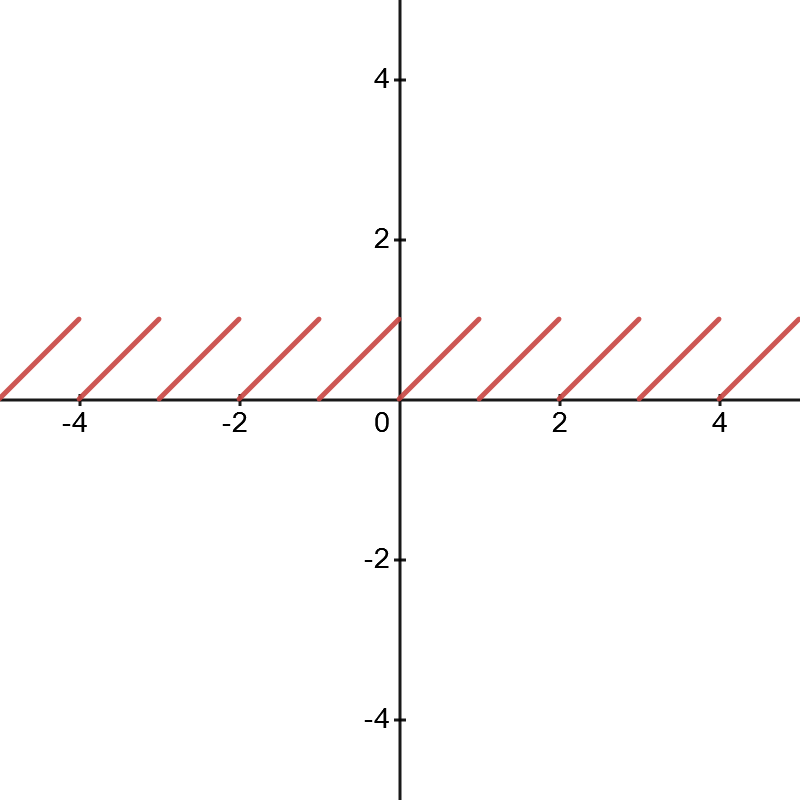
\includegraphics[width=0.5\textwidth]{fractionalfunction1.png} \\
Clearly, $f:\R \rightarrow [0,1)$ and $f$ is a surjection. Consider any interval $[n,n+1), \ \forall n \in \Z$. $f$ is strictly increasing on this interval because for any $x<y \in [n,n+1)$, the fractional part of $y$ is always greater than the fractional part of $x$. This functions is also the same as $g: \R \rightarrow [0,1), \ g(x):= x \text{ mod 1}$. Because $f(x) = f(x+1)$ for all $x \in \R$, $f$ is 1-periodic. \\
\bigskip
b) \\
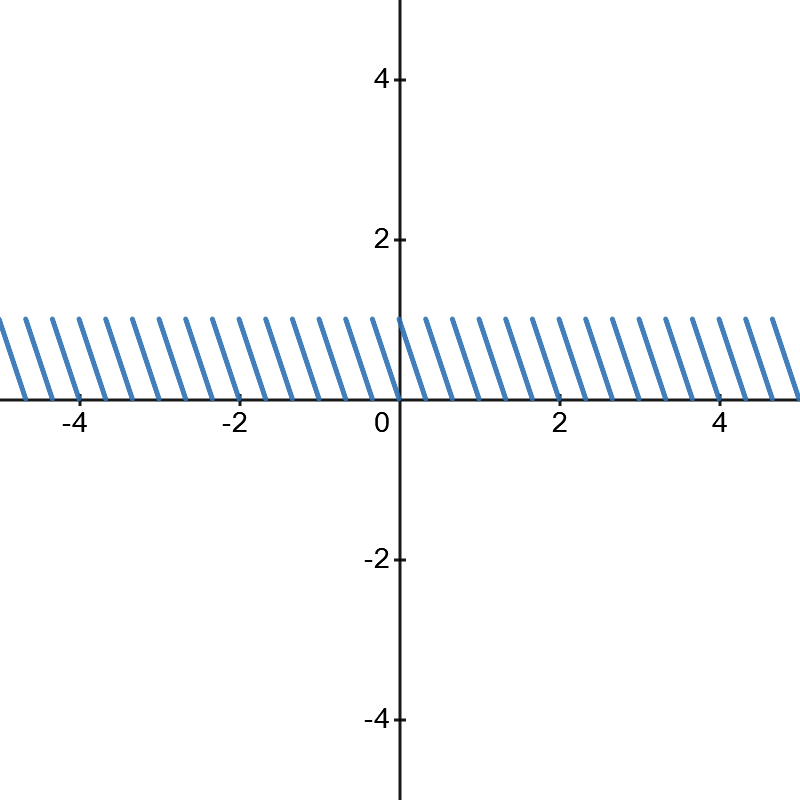
\includegraphics[width=0.5\textwidth]{fractionalfunction2.png} \\
This function is almost the same as the first, except it is horizontally compressed by a factor of 3 and flipped vertically because it is multiplied by -3. Because it is horizontally compressed by a factor of 3, then the function is strictly decreasing on the interval $[a\frac{n}{3}, a\frac{n}{3} + \frac{1}{3}), \forall n \in \Z \text{ and } \forall a \in \{ 0, 1, 2 \}$. Because $f(x) = f(x+\frac{1}{3})$ for all $x \in \R$, $f$ is $\frac{1}{3}$-periodic. \\
\bigskip
c) \\
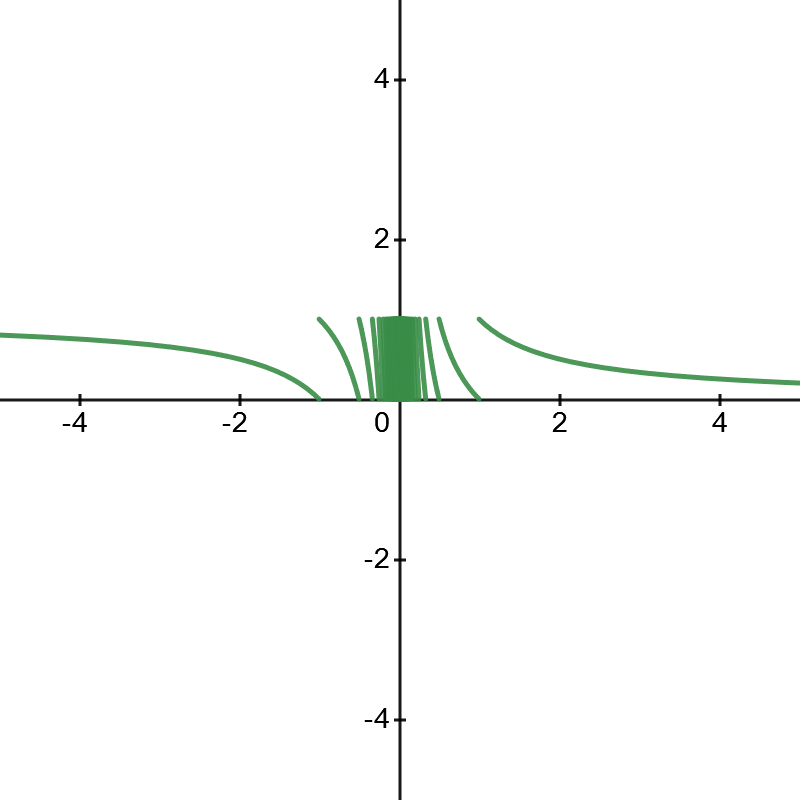
\includegraphics[width=0.5\textwidth]{fractionalfunction3.png} \\
This function is very different from the first two because it is not just a scalar multiple of the first function. If $x > 1$ then $f(\frac{1}{x}) < 1$ and strictly decreasing. But because $\frac{1}{x} < 1$ then $x=f(\frac{1}{x}), \ \forall x > 1$. A similar thing happens if $x < -1$. If $x \in (-1,1) \setminus \{ 0 \}$, then as $x$ gets closer to zero, $\frac{1}{x}$ grows reciprocally. Because $g:\R \setminus \{ 0 \} \rightarrow \R, \ g(x):= \frac{1}{x}$ is strictly decreasing, all intervals of $(\frac{1}{n}, \frac{1}{n+1}], \ \forall n \in \N: -1<\frac{1}{n}<1$ are strictly decreasing, and as $\frac{1}{n}$ gets closer to 0, these intervals get arbitrarily small. That is why you see this area near zero where the lines almost do not look separated.
\newpage

3.

\begin{myproof}
$\Rightarrow$ \\
Let $A$ be closed. For the sake of contradiction assume that there exists a limit point of $A$, $a$ such that $a \notin A$. Because $a$ is a limit point of $A$:
\begin{align*}
\forall \epsilon > 0 \exists x \in A: 0< |x-a|< \epsilon
\end{align*}
Consider we choose some $b \in A$ such that $b := x$. Since $A$ is closed, then $A^c$ is open:
\begin{align*}
\forall c \in A^c \exists \epsilon > 0 \forall y \in \R: |c-y| < \epsilon \implies y \in A^c
\end{align*}
Because we are assuming that $a \in A^c$, then we can choose $c := a$ and $y := b$. By $a$ being a limit point of $A$, $|b-a|=|a-b|< \epsilon $ meaning that $|c-y| < \epsilon$. This implies that $y =b$ is in $A^c$, but we specifically chose $b$ such that $b \in A$. Hence, this a contradiction. \\
\bigskip
Therefore, we have shown that if $A$ is closed, then $A$ contains all of its limit points. \\
\bigskip
$\Leftarrow$ \\
We will prove the contrapositive. Assume that $A$ is not closed, then $A^c$ is not open. Thus:
\begin{align*}
\exists x \in A^c \forall \epsilon >0 \exists y \in R: |x-y|<\epsilon \text{ and } y \notin A^c
\end{align*}
If $y \notin A^c$ then $y \in A$. Thus, $\forall \epsilon > 0: |x-y| < \epsilon$, and because $y \in A$, $x$ is a limit point of $A$. However, by assumption, $x \in A^c$. Thus, $A$ does not contain all of its limit points. \\
\bigskip
Therefore, if $A$ contains all of its limits points, then $A$ is closed.

\end{myproof}

\newpage

4. a)
\begin{myproof}
Because $f(x) \leq g(x) \leq h(x), \ \forall x \in A$, then $f(x) - \ell \leq g(x) - \ell \leq h(x) - \ell$. For any $\epsilon > 0$ we can choose a $\delta_1 > 0$ such that if $|x-a|<\delta_1 \implies |f(x) - \ell| < \epsilon$. We can also choose a $\delta_2 > 0$ such that if $|x-a|< \delta_2 \implies |h(x) -\ell| < \epsilon$. Suppose we chose $\delta := \text{ min}\{ \delta_1 , \delta_2 \}$. Thus if $|x-a| < \delta \implies$ 
\begin{align*}
-\epsilon < f(x) - \ell \leq & \ g(x) - \ell \leq h(x) - \ell < \epsilon \\
-\epsilon < & \ g(x) - \ell < \epsilon \\
& |g(x) - \ell| < \epsilon
\end{align*}
Therefore, $\lim_{x\to a} g(x) = \ell$.
\end{myproof}

b)

\begin{myproof}
By assumption, $\forall \epsilon_1 > 0 \exists \delta_1 > 0 \forall x \in A: 0 < |x-a| < \delta_1 \implies |f(x) - \ell| < \epsilon_1$ and $\forall \epsilon_2 > 0 \exists \delta_2 > 0 \forall x \in A: 0 < |x-a| < \delta_2 \implies |g(x) - m| < \epsilon_2$. \\
\bigskip
Suppose that max$\{ \ell, m \} = \ell$.\\
$\forall \epsilon > 0 \exists \delta' := \text{ min}\{\delta_1, \delta_2 \} \forall x \in A:|x-a|< \delta' \implies |f(x)- \ell| < \epsilon \text{ and } |g(x) - m| < \epsilon$. \\
Assume for the sake of contradiction $\exists \epsilon > 0 \forall 0< \delta \leq \delta':f(x) < g(x), \ \forall x \in (a-\delta, a+\delta)$. Let $\kappa:=$ min$(g(x)-f(x))$ on $(a-\delta, a+\delta)$. Notice that $\kappa > 0$ because $g(x) > f(x), \ \forall x \in (a-\delta, a+\delta)$. Choose $\epsilon'$ such that $\epsilon' < \text{ min}\{ \epsilon, \kappa \}$.  This implies that:
\begin{align*}
|f(x) - \ell | < & \frac{\epsilon'}{2} \\
|g(x) - m| < & \frac{\epsilon'}{2} \\
|g(x) -  | + |f(x) - \ell| < & \epsilon' \\
|g(x) - f(x) + \ell - m| \leq & |f(x) - \ell | + |g(x) - m| \\
|\kappa + \ell -m| \leq & |g(x) - f(x) + \ell - m| &  \\
-\epsilon < \kappa + \ell -m < & \epsilon' \\
\kappa - \epsilon + \ell < & m , \ \kappa - \epsilon' > 0
\end{align*}
This is a contradiction because max$\{ \ell, m\} = \ell$. Thus, $\forall \epsilon > 0 \exists 0< \delta \leq \delta': f(x) \geq g(x), \ \forall x \in (a - \delta, a+ \delta)$. If $|x-a| < \delta$ then $|$max$\{ f(x), g(x) \} - \text{ max}\{ \ell, m \}| = |f(x) - \ell| < \epsilon$ \\
\bigskip
We can make a similar case if max$\{ \ell, m \} = m$, where we simply says that there is some $\epsilon$-interval where $g(x) \geq f(x)$ for all $x$ in the interval. \\
\bigskip
Therefore, $\lim_{x\to a} \text{ max}\{ f(x), g(x) \} = \text{ max}\{ \ell, m \}$.

\end{myproof}
\newpage

5.
\begin{myproof}
$\Rightarrow$ \\
Consider $\forall \epsilon > 0 \exists \delta > 0 \forall x \in A: 0 < |x-a| < \delta \implies |f(x) - \ell | < \epsilon$ and $U \subseteq \R$ is open and $\ell \in U$. We will claim that there exists some $\epsilon > 0$ such that $(\ell - \epsilon, \ell + \epsilon) \subseteq U$. Consider this is false, and $\{ \ell \} \subseteq U$, but $(\ell - \epsilon, \ell + \epsilon) \not\subseteq U, \ \forall \epsilon > 0$, then $\{ \ell \} \notin U^c$, but $\ell$ is a limit point of $U^c$. This means that $U^c$ does not contain all of its limit points, making it not closed, meaning that $U$ is not open, a contradiction. Therefore, we can follow along with the existence of an $\epsilon >0$ such that $(\ell - \epsilon, \ell + \epsilon) \subseteq U$. Because $\forall \epsilon > 0 \exists \delta > 0 \forall x \in A: 0 < |x-a| < \delta \implies |f(x) - \ell | < \epsilon$ we can simply choose $V := (a - \delta, a + \delta)$. Thus, $V$ is open and $f((V \cap A) \setminus \{ a \} )  \subseteq U$. \\
\bigskip
Therefore, if $\lim_{x\to a}f(x) = \ell$ then $\forall U \subseteq \R \exists V \subseteq \R: U \text{ is open and } \ell \in U \implies V \text{ is open and } a \in V \text{ and } f((V \cap A) \setminus \{ a \}) \subseteq U$. \\
\bigskip
$\Leftarrow$ \\
Consider that $\forall U \subseteq \R \exists V \subseteq \R: U \text{ is open and } \ell \in U \implies V \text{ is open and } a \in V \text{ and } f((V \cap A) \setminus \{ a \}) \subseteq U$.
Consider $U := (\ell - \epsilon, \ell + \epsilon), \ \forall \epsilon > 0$. Then there exists some $V$ such that $a \in V$ and $V$ is open and $f((V \cap A) \setminus \{ a \}) \subseteq U$. We will claim that there exists some $\delta > 0$ such that $(a - \delta, a + \delta) \subseteq V$. Consider that this is false, and $\{ a \} \subseteq V$, but $(a - \delta, a + \delta) \not\subseteq V, \ \forall \delta > 0$, then $\{ a \} \notin V^c$, but $a$ is a limit point of $V^c$. This means that $V^c$ does not contain all of its limit points, meaning $V$ is not open, a contradiction. Thus, $\exists \delta > 0$ such that $(a - \delta, a + \delta) \subseteq V$. Because our choice of $\epsilon$ was arbitrary, we can now choose this $\delta$ to prove that $\forall \epsilon > 0 \exists \delta > 0 \forall x \in \R: 0 < |x-a| < \delta \implies |f(x)-\ell| < \epsilon$. \\
\bigskip
Therefore, if $\forall U \subseteq \R \exists V \subseteq \R: U \text{ is open and } \ell \in U \implies V \text{ is open and } a \in V \text{ and } f((V \cap A) \setminus \{ a \}) \subseteq U$ then $\lim_{x\to a}f(x) = \ell$.
\end{myproof}
\end{flushleft}
\end{document}